\chapter{Introduction}
\label{chap:intro}

\section{Biology of \Nsm{}}
\Nsm{} is a Gram-negative, bean-shaped diplococcal bacterium\cite{Deuren2000}, surrounded by a lipid membrane containing outer membrane proteins and lipopolysaccharides\cite{Deuren2000}. When pathogenic, the bacteria also has a polysaccharide capsule attached to the membrane\cite{Deuren2000}. It is non-spore forming, non-motile but piliated, and lives as an obligate human pathogen (humans being its only host)\cite{Stephens2009}. \Nm{} inhabits the mucosal membranes primarily in the respiratory tract, and it is estimated that up to 20-25\% of the population have this bacteria in their nasopharynx while being asymptomatic\cite{Rosenstein2001,Stephens2009,DeVoe1982}.

The \textit{Neisseria} genus contains a number of non-pathogenic species which are part of the normal human flora including \textit{N. subflava},  \textit{N. flavescens},  \textit{N. lactamica} and \textit{N. sicca}\cite{Aas2005}. Two species of \textit{Neisseria} are the causative agents of human diseases, \Nm{}, which causes bacterial meningitis and \textit{N. gonorrhoea} which causes gonorrhoea. Being $\beta$-proteobacteria\cite{Stephens2009}, the \textit{Neisseria} genus is also related to a number of other pathogenic bacteria including \textit{Bordetella}, \textit{Burkholderia} and \textit{Spirillum}. This taxa also includes ammonia-oxidising bacteria such as \textit{Nitrosomonas}\cite{Madigan2005}, .

\Nm{} is classified into 13 different serogroups based on the differences in lipopolysaccharides, capsules, outer membrane proteins and adhesion molecules\cite{Stephens2009,Deuren2000,Carbonnelle2009}. 3 of these 13 serogroups are the main cause of meningococcal meningitis, with serogroups B and C being the most prevalent\cite{Deuren2000}. Vaccines for serogroup C are available, but serogroup B currently has no effective vaccine, as it mimics human antigens\cite{Stephens2009} and it is a poor immunogen\cite{Stephens2007}. In addition to being the causative agent for meningococcal meningitis, \Nm{} also causes septicaemia and the combination has a mortality rate of ~10\% even with therapy\cite{Deuren2000,Stephens2009}.

\Nm{} is dependent on a source of iron, and must source this from its environment\cite{Larson2002}. It does this by directly capturing iron from the host via human transferrins\cite{Archibald1978,Perkins-Balding2004,Larson2002} and lactoferrin\cite{Larson2002}. This capture is brought about by membrane surface receptors that can bind the transferrins which then go on to internalise the iron into the bacterium for growth\cite{Yazdankhah2004}.

\section{Pathogenicity of \Nm{}}
Meningitis is caused by \Nm{} entering the bloodstream and travelling to the meninges, a set of membranes that envelope the central nervous system, where the bacteria goes on to cause inflammation. Once it has entered the bloodstream, \Nm{} is capable of switching its capsule by phase-variation to avoid host-immune detection\cite{Beddek2009,Moxon1994}. After colonisation by the bacterium, in order to enter the bloodstream, it must first adhere to the mucosal tissue. This is facilitated by adhesion molecules on the outer membrane and by pili, with the latter being the primary source of adhesion\cite{Deuren2000,Carbonnelle2009}. Once the bacteria are adhered to the mucosal cells, additional contacts are made with the outer membrane proteins. Interestingly, the presence of the polysaccharide capsule, which is required for survival in the bloodstream, interferes with these additional contacts\cite{Stephens2009}. \Nm{} invades the bloodstream by being endocytosed by the mucosal epithelial cells, a process which is triggered by the pili and outer membrane proteins on the bacteria.

\Nm{} is able to survive in the bloodstream (typically an antimicrobial environment) mainly by virtue of its polysaccharide capsule as this is able to protect the bacteria against various immune responses by the host including complement-mediated bacteriolysis and phagocytosis by neutrophils\cite{Deuren2000}. Despite these protective features, specific antibodies \textit{do} provide full protection against the bacteria, but the time taken for these antibodies to be produced means that the host has a period of at least 1 week in which it must rely on innate immune response\cite{Deuren2000}. Evidence suggests that systemic infection by \Nm{} can only occur in hosts which are immunocompromised in some way, specifically if they do not have the serum bactericidal antibodies against capsular or non-capsular antigens, or they are missing certain complement components\cite{DeVoe1982}. A number of factors can increase the likelihood of contracting bacterial meningitis including smoking and travelling to epidemic regions\cite{Stephens2009}. In developed countries, the highest rates of invasive meningococcal meningitis are seen in infants and children less than 4 years-old, adolescents, military recruits and groups where crowding and new exposures occur such as college students living in dormitories, however the disease is capable of affecting all age groups\cite{Stephens2009}.

There is evidence to suggest that much of the damage done to the host during a meningococcal infection is actually caused by the host in an attempt to rid itself of the bacteria\cite{Pathan2003}. A systemic infection causes a massive inflammatory response and the resulting quantities of cytokines produced eventually lead to organ dysfunction and the proteases produced by neutrophil activation also lead to endothelial injury\cite{Pathan2003}.

Once \Nm{} has entered the bloodstream, it goes on to invade the cerebro-spinal fluid (CSF\nomenclature{CSF}{Cerebrospinal Fluid}), which serves as an excellent culture medium for the bacteria\cite{DeVoe1982}. The host response to this infection is inflammation of the meninges, the membranes surrounding the central nervous system. This leads to a build-up of serous fluid in the brain causing cerebral swelling. Once the bacteria have entered the CSF, antimicrobial treatment is required otherwise the effects are almost invariably fatal\cite{DeVoe1982}.

Initially a meningococcal infection presents as a slight fever and chills, which may improve after 4-6 hours. Haemorrhagic skins lesions may appears between 8 and 18 hours, however roughly 20\% of suffers never present with lesions. These skin lesions are possibly the most well known symptom of bacterial meningitis as they are characterised by a non-blanching (does not turn white under mild pressure) rash. The clearest evidence for meningococcal infection is a fever, stiff neck, aversion to bright light, vomiting, skin lesions and headaches. Unfortunately not all these symptoms may be present in all cases\cite{DeVoe1982}.

When meningococcal septicaemia occurs, renal function may be impaired as a direct consequence of cardiac impairment. Septicaemia causes ``capillary leak'' which reduces cardiac output and increases the effort required to breathe normally. Reduced cardiac output can also affect the gastrointestinal tract leading to reduced function. Once treated these symptoms will usually subside as cardiac output improves\cite{Pathan2003}.

In most cases the treatment for meningococcal meningitis is with antibiotics, where the primary aim is to achieve a rapid bactericidal effect in the CSF\cite{Deuren2000}. This treatment is suggested prior to positive identification of cultures of the bacteria obtained from the CSF as any delay is potentially life-threatening if the bacteria have indeed invaded the CSF\cite{DeVoe1982}.

\section{Growth of \Nm{}}
Bacteria require carbon and energy sources in order to grow, and these are often sourced from sugars present in the environment. \Nm{} can only use the sugars glucose and maltose as carbon sources\cite{Exley2005,Beno1968}, however they can use peptides as carbon sources. The bacteria are usually grown on M\"uller-Hinton broth and Columbia agar which are peptide-based formulations. 

\section{Organisation of the Respiratory Chain of \Nm{}}
\Nm{} is classified as an aerobe and as such has an oxidase pathway for reducing oxygen (\cOxygen{}), but given that the environment in the nasopharynx is poor in oxygen, the bacteria must also be capable of respiring in a microaerobic environment. This is evidenced by the fact that bacterial isolates from the nasopharynx routinely contain both strict aerobes and strict anaerobes\cite{Rock2005}. Genomic analysis of 2 strains of \Nm{} shows that there are 3 terminal oxidases; 1 of each for reducing oxygen, nitrite (\cNitrite{}) and nitric oxide (\cNO{})\cite{Rock2005a}. This analysis may be expanded as there are now many more genomes published. Experiments showed that under oxygen limiting conditions, \Nm{} was capable of growth when nitrite was present in the media (M\"uller-Hinton Broth), and that nitrate (NO$_{\textrm{3}}^{\textrm{-}}$), the probable source for nitrite, had no effect on growth\cite{Rock2005a}. Additionally the bacteria require carbon dioxide, as shown by \citet{Tuttle1952} and have 2 enzymes which catalyse the reduction of CO$_{\textrm{2}}$\cite{DeVoe1982}.

\textit{In vivo}, nitrite is obtained as a product of digesting nitrate in food. There are a number of facultative nitrate-reducing bacteria present in the mouth and pharynx responsible for this\cite{Rock2005} which additionally have a proposed benefit of protecting the host against peridontal and cariogenic bacteria\cite{Lundberg2004}. Nitrite is also created by oxidation of nitric oxide, which is produced as a host signalling molecule and as a toxin as part of the host immune response\cite{Lundberg2004,Rock2005}.

The respiratory pathway for reducing nitrite in \Nm{} involves two steps; nitrite is reduced to nitric oxide, which is then further reduced to nitrous oxide. This represents incomplete reduction, as a further reduction step is possible (shown in Figure \ref{fig:completedenitrification}), reducing nitrous oxide to dinitrogen gas\cite{Rock2005,Deeudom2006}.

\begin{figure}[tbp]
	\begin{center}
	\colorbox{LightBlue}{$\mathrm{NO}_3^-\rightarrow$}$\mathrm{NO}_2^-\rightarrow\mathrm{NO}\rightarrow\mathrm{N}_2\mathrm{O}$\colorbox{LightBlue}{$\rightarrow\mathrm{N}_2$}
	\caption[{Complete denitrification.}]{{\bf Complete denitrification.} The process of reducing nitrite to nitrogen gas. In \Nm{} the first and final steps highlighted in blue do not occur.
	\label{fig:completedenitrification}}
	\end{center}
\end{figure}

Reduction of oxygen is favourable over nitrite reduction due to the redox potential differences. The redox potential of \cOxygen{}/H$_{\textrm{2}}$O is $+820$ mV, \cNitrite{}/\cNO{} is $+348$ mV, thus \cOxygen{} has a higher tendency to acquire electrons resulting in a electrochemically favourable reaction\cite{Deeudom2007}. The electron flow towards the oxidase is also preferred physiologically as it liberates more energy by virtue of the translocation of more protons than the reduction of nitrite. The translocated protons are ultimately used in the synthesis of ATP\nomenclature{ATP}{Adenosine triphosphate} molecules for energy. This results in reduction of oxygen in preference to nitrite when both are present (in most cases).

Reduction of oxygen in \Nm{} is carried out by the oxygen reductase cytochrome \cbbthree{} oxidase, a membrane-bound heme-copper oxidase\cite{Preisig1996}. \cbbthree{} is capable of binding oxygen and nitric oxide, which means that during nitrite reduction (denitrification), the oxidase can be competitively inhibited (chemically) by the intermediate product of denitrification. \cbbthree{} can be permanently damaged at high concentrations of \cNO{} and \cOxygen{}, as they can both bind at the \cbbthree{} active site and react together to form peroxynitrite\cite{Brown1994,Sharpe1998,Anjum2002}.

Nitrite is reduced by the nitrite reductase AniA\nomenclature{AniA}{Anaerobically inducible protein A from \textit{Neisseria} sp.}, which is a copper containing reductase. This reduction does not involve translocation of protons, and thus does not produce any usable energy. Nitrite is reduced to nitric oxide which can then be further reduced by a nitric oxide reductase NorB. Since \Nm{} is capable of reducing nitric oxide, a host toxin, directly, this may help it defend itself against part of the host immune response\cite{Heurlier2008,Rock2005} as has been shown in tissue culture by \citet{Anjum2002}.

The reduction processes carried out by these enzymes are shown in the table in Table ~{\ref{tab:reduction-enzymes}}.

\begin{table}[tbp]
\begin{center}
\begin{tabular}{lclc}
\toprule
\multicolumn{3}{c}{\textbf{Reduction}}& \textbf{Enzyme} \\
\midrule
\cNitrite{} & $\rightarrow$ & \cNO{} & AniA \\
\cNO{} & $\rightarrow$ & \cNtwoO{} & NorB \\
\cOxygen{} & $\rightarrow$ & H$_{\textrm{2}}$O & \cbbthree{} \\
\bottomrule
\end{tabular} 
\end{center}
\caption{The reductions catalysed by the respiratory enzymes in \Nm{}
\label{tab:reduction-enzymes}}
\end{table}

The major source for electrons in both respiratory pathways is NADH\nomenclature{NADH}{Nicotinamide adenine dinucleotide}, although electrons can also be obtained from pyruvate and lactate amongst others. These reduced substrates lead to reduction of ubiquinone to ubiquinol in the ubiquinone pool that exists within the bacteria. Ubiquinol is oxidised either by the cytochrome \textit{bc$_{\textrm{1}}$} complex or directly by the NorB\nomenclature{NorB}{Nitric Oxide Reductase B from \textit{Neisseria} sp.} enzyme whilst reducing \cNO{} to \cNtwoO{}. Cytochrome \textit{bc$_{\textrm{1}}$} is oxidised by a number of intermediate cytochromes which act to transport electrons to the terminal oxidases; AniA and \cbbthree{}. The \textit{c$_{\textrm{5}}$} cytochrome transports electrons from the \textit{bc$_{\textrm{1}}$} complex to AniA, and two cytochromes, \textit{c$_{\textrm{2/x}}$} and \textit{c$_{\textrm{4}}$}, transport electrons to \cbbthree{}. It is not understood why \cbbthree{} has 2 alternate cytochromes, and there is evidence to suggest that it can also be supplied, in a limited capacity, by the \textit{c$_{\textrm{5}}$} cytochrome as well\cite{Deeudom2008}. The electron transport chain is shown graphically in Figure \ref{fig:etc}.

\begin{figure}[tbp]
 \begin{center}
 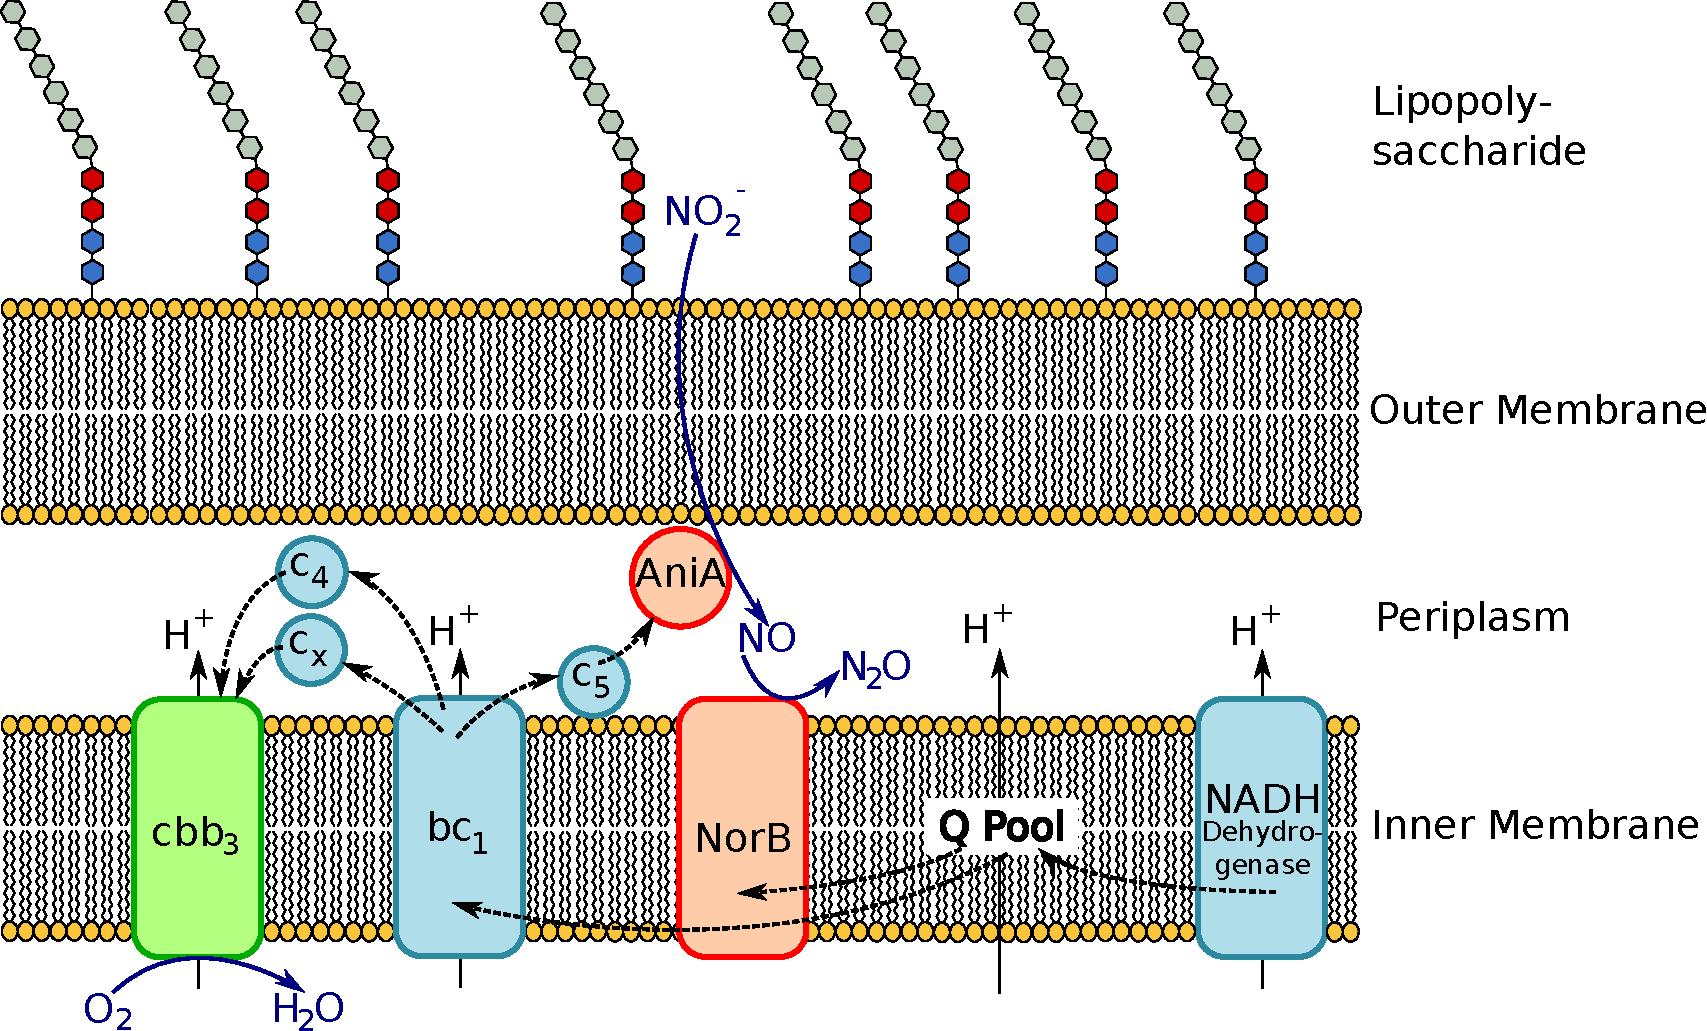
\includegraphics[width=14cm]{./01-introduction/data/Respiratory_layout.pdf}
 % Respiratory_layout.pdf: 819x404 pixel, 72dpi, 28.89x14.25 cm, bb=0 0 819 404
\end{center}
\caption[{Layout of the components of the respiratory system in \Nsm{}.}]{{\bf Layout of the components of the respiratory system in \Nsm{}.} Oxygen reducing components are shown in green, nitrogen reducing components in red. Components transporting electrons are coloured light blue, and their transport is indicated by dashed arrows. Respiratory substrates are shown in dark blue, with corresponding arrows linking them to their reducing enzymes. Components which produce membrane potential are also indicated.
\label{fig:etc}}
\end{figure}

In addition to the difference in favourability between the two respiratory pathways, there is also a great deal of regulation, both at the enzymatic and transcriptional level. Chemical inhibition also plays a part in regulation as briefly mentioned previously. Expression of AniA is regulated by two processes, the reduction of oxygen and the presence of nitrite. The presence of oxygen down-regulates the expression of an activator of AniA expression. This activator is FNR (fumarate and nitrate reduction regulator)\nomenclature{FNR}{Fumarate and Nitrite reduction Regulator}, and the presence of oxygen effectively means that AniA expression is repressed by the reduced expression of FNR. In \Nm{}, FNR appears to work slightly differently than in facultative anaerobes such as \textit{E. coli}, in that FNR is still expressed at quite high concentrations of oxygen, and is itself down-regulated by a separate co-factor\cite{Rock2007}.

The presence of nitrite triggers the two component NarP/NarQ\nomenclature{NarP}{Nitrate/Nitrite Response Regulator}\nomenclature{NarQ}{Nitrate/Nitrite Response Sensor} system which activates expression of AniA in response to increasing levels of nitrite\cite{Rock2005}. The activity of AniA is also controlled by the competition for electrons by the other reductase enzymes in the respiratory chain. Both NorB and \cbbthree{} have a higher affinity for electrons than AniA, and as a result the presence of these enzymes (when active) has an inhibitory effect on AniA. The regulation of AniA is further complicated by the production of nitric oxide, and the presence of a protein, NsrR\nomenclature{NsrR}{Nitrite sensing repressor protein}.

Nitric oxide has a direct inhibitory effect on the expression of AniA, as does the NsrR protein. Nitric oxide also inhibits the NsrR protein, leading to a de-represssion of AniA\cite{Heurlier2008}. In the absence of nitric oxide, AniA is almost fully repressed by active NsrR. As \cNO{} concentrations increase, NsrR is inactivated allowing full activation of AniA. Once \cNO{} reaches a sufficiently high level it will begin to inhibit AniA\cite{Rock2005,Rock2007}.

NorB is less tightly regulated by respiratory components, as it is only acted upon by NsrR, however it is regulated by FNR and NrsR outside the respiratory chain\cite{Isabella2008}. This regulation by NsrR works in a similar way to how NsrR acts upon AniA. When there is no nitric oxide present, the NsrR acts to inhibit NorB since there is no substrate for it to reduce. In the presence of nitric oxide, NsrR is inhibited, leading to the activation of NorB which is now able to reduce \cNO{} to \cNtwoO{}. In this case nitric oxide is acting as a de-repressor of NorB.

This complicated set of regulatory relationships between the different components of the respiratory pathways is shown in Figure \ref{fig:respiratory-pathway}.

\begin{figure}[tbp]
 \begin{center}
 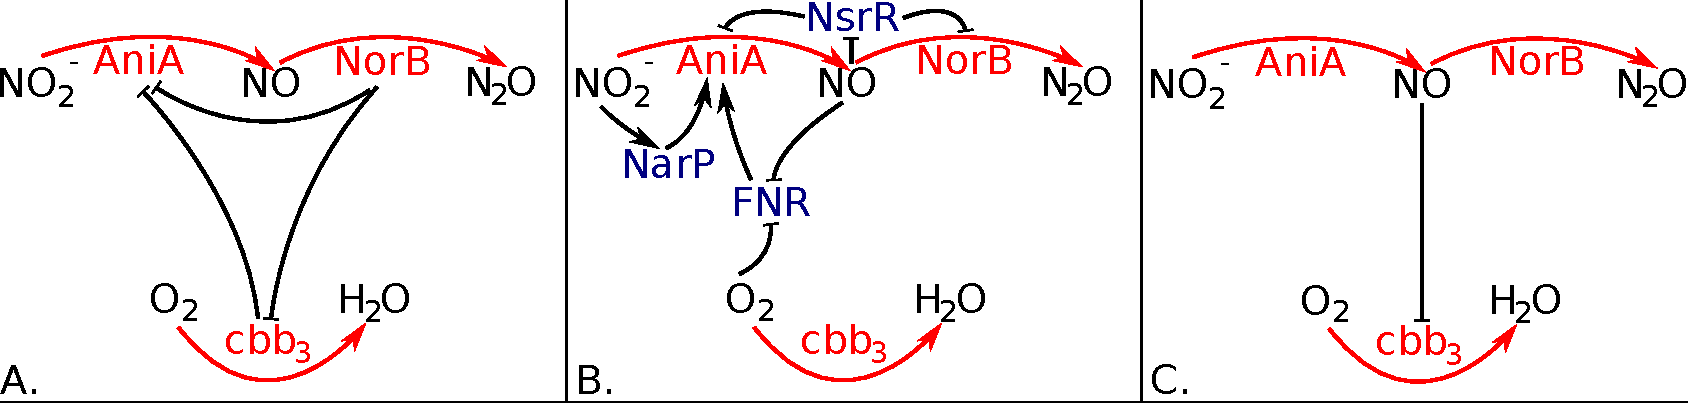
\includegraphics[width=14cm]{./01-introduction/data/regulation.pdf}
\end{center}
\caption[{Regulation of respiratory components in \Nsm{}.}]{{\bf Regulation of respiratory components in \Nsm{}.} Enzymes and enzymatic reactions are shown in red. \textit{A.} describes the regulation caused by competition for electrons between the respiratory enzymes. \textit{B.} shows the genetic regulation, which also involves a number of additional components in dark blue. \textit{C.} shows chemical inhibition of the respiratory components.
\label{fig:respiratory-pathway}}
\end{figure}

\section{Respiratory Enzymes in \Nm{}}
\subsection{Cytochrome \cbbthree{} oxidase}
Cytochrome \cbbthree{} oxidase is a Haem Copper Oxidase (HCO)\nomenclature{HCO}{Haem Copper Oxidase} enzyme found commonly in proteobacteria. They have been characterised in at least \textit{Pseudomonas denitrificans}, \textit{Rhodobacter sphaeroides}, \textit{Rhodobacter capsulatus} and \textit{Bradyrhizobium japonicum}\cite{Pitcher2004}. HCOs catalyse the reduction of Oxygen molecules to water whilst translocating protons across the inner membrane, from the cytoplasm to the periplasm, producing an electrochemical gradient.

HCOs can be separated into two categories by their electron donor type. Cytochrome \textit{c} oxidases accept electrons from \textit{c}-type cytochromes, and quinol oxidases accept electrons from ubiquinol. The major difference between these two categories is a missing $\mathrm{Cu}_\mathrm{A}$ site in quinol oxidases\cite{Puustinen1996}. HCOs can be further broken down to 3 type, the $\mathit{aa}_3$-type cytochrome \textit{c} oxidase, the $\mathit{bo}_3$-type quinol oxidase and the \cbbthree{}-type cytochrome \textit{c} oxidase\cite{vanderOost1994}. Alternatively 5 different HCO subclasses may be classified, the $\mathit{aa}_3$, $\mathit{caa}_3$ and \cbbthree{}-type cytochrome \textit{c} oxidases, and the $\mathit{bo}_3$ and $\mathit{aa}_3$-type quinol oxidases\cite{Garcia-Horsman1994}. All of these different types of cytochrome \textit{c} oxidases are found in bacteria, whereas those in mitochondria are limited to $\mathit{aa}_3$-type cytochrome \textit{c} oxidases\cite{Keilin1939}.

HCOs are themselves ``defined by the primary sequence of their catalytic subunit, which is composed of twelve transmembrane helices with six invariant histidines ligating three cofactors; a high spin heme (one His ligand) and a copper (3 His ligands) in the catalytic site and an additional low-spin heme (two His ligands)''\cite{Huang2010}. Sequence alignment has also indicated that bacterial NO-reductase (NOR)\nomenclature{NOR}{Nitric Oxide Reductase} might also be a divergent member of the HCO family. A schematic diagram of the \cbbthree{} oxidase is shown in Figure \ref{fig:cbb3}. \cbbthree{} is composed of three main subunits with CcoN being the catalytic subunit, which is related to subunit I of $\mathit{aa}_3$ oxidases and NorB. This latter relation to NorB explains why \cbbthree{} has some Nitric Oxide reduction activity (and conversely why NorB has some Oxygen reduction activity)\cite{Huang2010}. CcoN contains the catalytic site \textendash{} the high-spin heme $\mathit{b}_3\mhyphen\mathrm{Cu}_{\mathrm{B}}$ \textendash{} and a low spin heme \textit{b}. CcoO is anchored in the inner membrane and contains just one \textit{c-type} heme. CcoP contains two \textit{c}-type hemes and is anchored to the inner membrane. CcoQ, the fourth subunit is small, and helps to stabilise the complex\cite{Huang2010}.

\begin{figure}[tbp]
	\begin{center}
		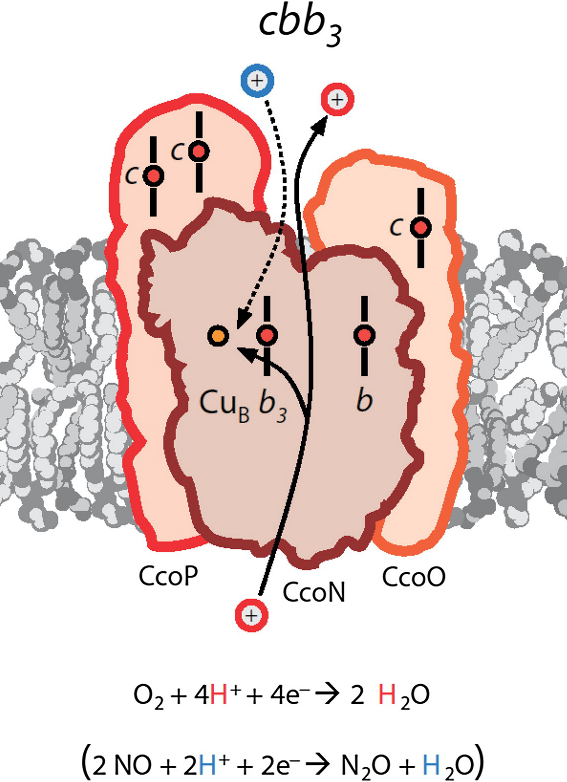
\includegraphics[height=10cm]{01-introduction/data/cbb3_only.png}
	\end{center}
	\caption[{The \cbbthree{} oxidase}.]{{\bf The \cbbthree{} oxidase}. This diagram shows the proton input pathway for Oxygen reduction shown in red, and the putative pathway for Nitric Oxide reduction in blue. Also shown are the 3 subunits and their associated heme centres. Adapted from \citet{Huang2010}.
	\label{fig:cbb3}}
\end{figure}

The mechanism of reduction of $\mathrm{O}_2$ by \cbbthree{} oxidases is not fully understood, as the reduction intermediates currently remain unknown\cite{Huang2010}. The cytochrome \cbbthree{} oxidases have very low $\mathrm{K}_\mathrm{m}$ values, allowing them to operate even under oxygen limiting conditions. \cbbthree{} from \textit{Bradyrhizobium japonicum} has a $\mathrm{K}_\mathrm{m}$ of 7 nM, much lower than that of the mitochondrial $aa_3$ oxidase\cite{Zufferey1996}. This high affinity for oxygen suggests that \Nm{} may have become adapted to surviving in the human host in areas of low oxygen concentration. Since this type of oxidase is also found in other human pathogens it is likely that it is used to allow those pathogens to survive in hypoxic environments in the human host\cite{Preisig1996a}.

The catalytic reaction for the \cbbthree{} oxidase is:
\begin{equation}
cbb_{3\mathrm{(reduced)}} + \tfrac{1}{2}\mathrm{O}_2 + 2\mathrm{H}^+ \rightarrow cbb_{3\mathrm{(oxidised)}} + \mathrm{H}_2\mathrm{O}
\end{equation}

\subsection{NorB Nitric Oxide Reductase}
Nitric Oxide Reductase is also a Haem Copper Oxidase enzyme which is found in bacteria as an integral membrane protein. There are three types of NOR, the cytochrome \textit{bc} type complex (cNOR), the cytochrome \textit{b} type complex lacking the cytochrome \textit{c} component (qNOR) and a qNOR-type reductase that also includes $\mathrm{Cu}_{\mathrm{A}}$ ($\mathrm{qCu}_{\mathrm{A}}\mathrm{NOR}$). cNOR-type reductases receive electrons from soluble redox protein donors, whereas qNOR-type reductases receive electrons from quinol\cite{Householder2000}.

The NOR in \Nm{} is a qNOR-type reductase, and is encoded by the norB gene (NMB1622). It catalyses the reduction of Nitric Oxide to Nitrous Oxide receiving electrons directly from the quinone pool. Under microaerobic conditions this enzyme is important as during dentrification to support growth, Nitric Oxide accumulates as a result of reduction of Nitrite. The build up of Nitric Oxide inhibits aerobic respiration as it binds competitively to the \cbbthree{} oxidase. NorB protects the bacteria from the toxicity extracellular NO which is produced by host tissues and macrophages, which produce NO in quantity during infection\cite{Heurlier2008}.

The nitric oxide reductase in \textit{Neisseria gonorrhoeae} is predicted to be an 84.3 kDa protein with significant sequence identity to \textit{Ralstonia eutropha} and consists only of the NorB subunit\cite{Householder2000}. The NorB protein is highly conserved across all \textit{Neisseria} species as evidenced by sequence analysis\cite{Barth2009}.

The catalytic reaction for NorB is:
\begin{equation}
\mathrm{NorB}_{\mathrm{(reduced)}} + 2\mathrm{NO} + 2\mathrm{H}^+ \rightarrow \mathrm{NorB}_{\mathrm{(oxidised)}} + \mathrm{N}_2\mathrm{O} + \mathrm{H}_2\mathrm{O}
\end{equation}

\subsection{AniA Nitrite Reductase}
AniA nitrite reductase is an anaerobically induced, outer membrane associated protein which uses nitrite as an electron acceptor\cite{Clark1987}. It is a copper-containing protein found in many denitrifying proteobacteria.

Nitrite reductases catalyse the reduction of nitrite to nitric oxide with no associated proton translocation. There are two types of nitrite reductase, those that have haem centres, and those which have copper centres. AniA in \Nm{} is a copper-containing and accepts electrons from \textit{c}-type cytochromes ($c_5$).

In \Nm{} this enzyme is important during oxygen limiting conditions as it allows microaerobic respiration which can supplement growth by denitrification\cite{Rock2005}.

Interestingly, according to its genome sequence \Nm{} strain 053442 appears to lack the \textit{aniA} gene in its entirety, suggesting that this strain would be unable to perform denitrification and respire anaerobically\cite{Barth2009}. 32\% of \Nm{} strains sequenced by \citet{Barth2009} contain non-functional copies of \textit{aniA} with frameshift mutations. These strains do still possess the \textit{norB} gene for reducing Nitric Oxide however allowing them to prevent its toxic effects. It has been suggested by some that this may actually be evidence that \Nsm{} is in the process of evolving away from denitrification to being a Nitric Oxide tolerant aerobe\cite{Moir2011}.

The catalytic reaction for AniA is:
\begin{equation}
\mathrm{AniA}_{\mathrm{(reduced)}} + \mathrm{NO}_2^- + 2\mathrm{H}^+ \rightarrow \mathrm{AniA}_{\mathrm{(oxidised)}} + \mathrm{NO} + \mathrm{H}_2\mathrm{O}
\end{equation}

\section{Respiratory Electron Transporters in \Nm{}}
\subsection{NADH Dehydrogenase}
NADH (Reduced Nicotinamide Adenine Dinucleotide) Dehydrogenase is an inner membrane bound enzyme that catalyses the transfer of electrons from NADH to the quinone pool in many bacteria. There are three types of NADH dehydrogenase enzymes found in bacteria, NDH-1, NDH-2 and $\mathrm{Na}^+$-NDH. NDH-1 is related to Complex I of the mitochondrial respiratory chain and translocated protons across the inner-membrane whilst reducing the quinone pool\cite{Weiss1991,Carroll2003,Friedrich2004}. NDH-2 does not have any proton pump activity, nor does it have any Fe-S clusters\cite{Yagi1991}. $\mathrm{Na}^+$-NDH translocates $\mathrm{Na}^+$ ions across the membrane\cite{Gemperli2002}. The NADH dehydrogenase of \Nm{} is of the NDH-1 type\cite{Deeudom2007}.

Mitochondrial complex I catalyses the oxidation of NADH and the reduction of ubiquinone whilst translocating 4 protons across the membrane. It does so using the following reaction scheme:
\begin{equation}
\mathrm{NADH} + \mathrm{H}^+ + 4\mathrm{H}^+_{\mathrm{inner}} + \mathrm{UQ} \rightarrow \mathrm{NAD}^+ + 4\mathrm{H}^+_{\mathrm{outer}} + \mathrm{UQH}_2
\end{equation}

\subsection{Cytochrome $bc_\mathrm{1}$ Complex}
The cytochrome $bc_\mathrm{1}$ complex oxidises quinols and reduces metalloprotein electron transporters (usually c-type cytochromes). It is an important part of bacterial respiratory chains, and is also analogous to the mitochondrial complex III\cite{Thoeny-Meyer1997}. Whilst catalysing the reduction of ubiquinol and the oxidation of c-type cytochromes, the $bc_\mathrm{1}$ complex also translocates protons across the inner membrane from the cytoplasm to the periplasm producing an electrochemical gradient. The $bc_\mathrm{1}$ complex is found in both Gram negative and Gram positive bacteria, however \textit{E. coli} has no $bc_\mathrm{1}$ complex. The homolg the $b_6f$ complex is also used for electron transfer during photosynthesis in higher plants and phototrophic bacteria\cite{Darrouzet1999}.

In bacteria the $bc_1$ complex is formed of one cyt \textit{b} subunit which contains two \textit{b}-type hemes, one cyt $c_1$ subunit which contains a single \textit{c}-type heme and an Rieske iron-sulfur protein. These subunits form the two catalytic sites of the $bc_1$ complex. The reduction of ubiquinol appears to occur in a concerted manner at 1 of these sites, $\mathrm{Q}_o$\cite{Darrouzet1999}. Electrons from the quinol are shared between two reaction chains, 1 which transfers electrons to the high-potential iron-sulfur protein and $c_1$, and another which transfers electrons to the low-potential cytochrome \textit{b}. The other catalytic site $\mathrm{Q}_i$ uses the two electrons from the high and low potential chains to reduce quinone, or other metalloprotein electron transporters\cite{Snyder2000,Berry2011}. This modified Q-cycle is shown in Figure \ref{fig:q-cycle}.

\begin{figure}[tbp]
	\begin{center}
		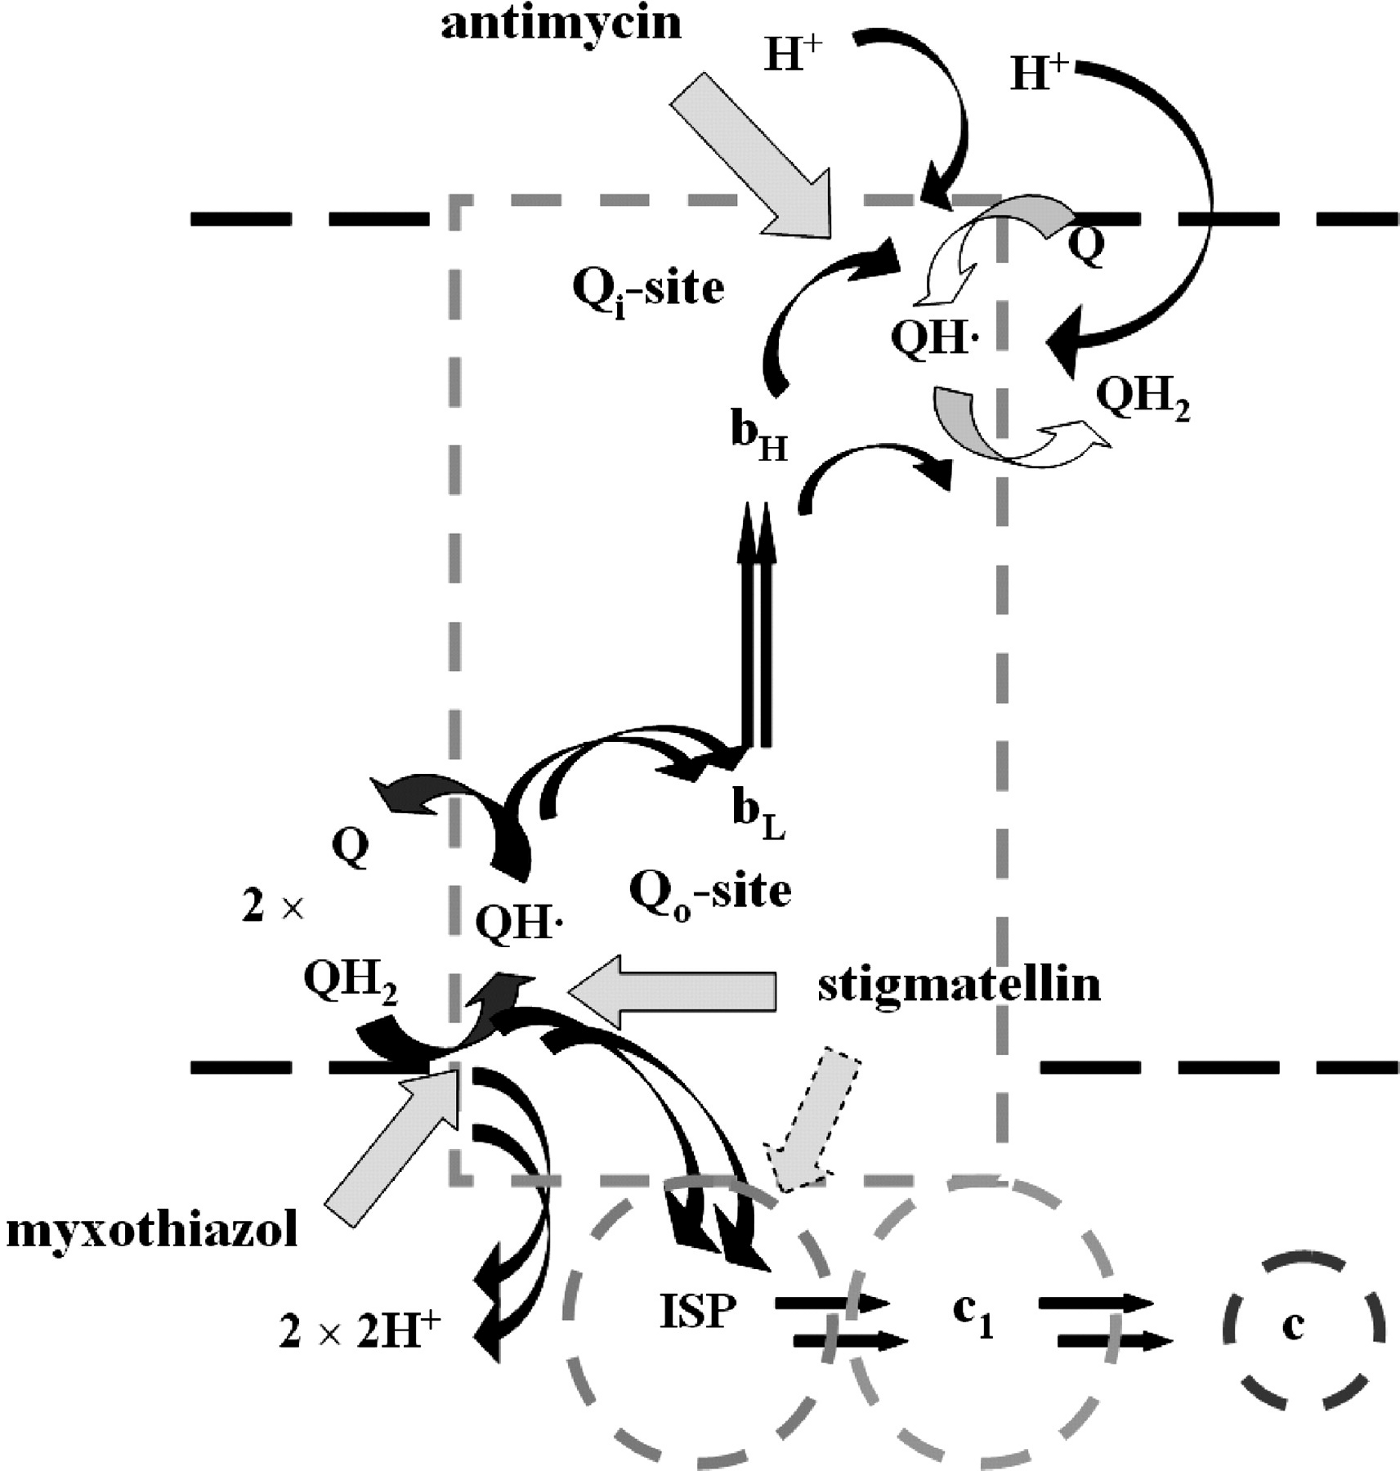
\includegraphics[width=14cm]{01-introduction/data/q-cycle.png}
	\caption[The modified Q-cycle used by the bacterial $bc_1$ complex.]{{\bf The modified Q-cycle used by the bacterial $bc_1$ complex.}  The cyt \textit{b} subunit is represented by the \textit{dashed gray} outline, and contains the $\mathrm{Q}_\mathrm{o}$- and $\mathrm{Q}_\mathrm{i}$-sites, connected by hemes $b_\mathrm{L}$ and $b_\mathrm{H}$. The ISP and cyt $c_1$ catalytic domains and cyt \textit{c} are represented by \textit{dashed darker gray circles}. Electron transfer steps are shown by \textit{dark narrow arrows,} proton release and uptake by \textit{lighter arrows}, binding and release of quinone species by \textit{broad curved arrows} (dark gray for $\mathrm{Q}_\mathrm{o}$-site, light gray for $\mathrm{Q}_\mathrm{i}$-site). Sites of inhibition are indicated by \textit{block arrows} showing sites at which the bound inhibitor displaces quinone species. The \textit{dashed inhibitor arrow} indicates that the reaction of ISPH with cyt $c_1$ is blocked by the interaction of ISPH with stigmatellin at the $\mathrm{Q}_\mathrm{o}$-site. Adapted from \citet{Crofts2003}.
	\label{fig:q-cycle}}
	\end{center}
\end{figure}

The reaction scheme for the $bc_1$ complex is:
\begin{equation}
\mathrm{QH}_2 + 2 \mathrm{~ferricyt~} c^{3+} + 2\mathrm{H}^+_{\mathrm{Negative}} \Longleftrightarrow \mathrm{Q} + 2 \mathrm{~ferrocyt~} c^{2+} + 4\mathrm{H}^+_{\mathrm{Positive}}
\end{equation}

\subsection{Cytochromes $c_\mathrm{4}$, $c_\mathrm{x}$ and $c_\mathrm{5}$}
Cytochromes $c_\mathrm{4}$, $c_\mathrm{x}$ and $c_\mathrm{5}$ are soluble \textit{c}-type cytochromes. These are small heme proteins that are found in the periplasm and are loosely associated with the inner membrane. Along with their presence in proteobacteria, the \textit{c}-type cytochromes also form part of the mitochondrial respiratory apparatus in the form of cytochrome \textit{c}. Bacterial \textit{c}-type cytochromes perform a very similar function to mitochondrial cytochrome \textit{c} in that they transport electrons from the $bc_1$ complex to the terminal reductases. Cytochromes \textit{c}-552, \textit{c}-553 \& \textit{c}-554 from algal chloroplasts and cyanobacteria, $c_2$ from purple photosynthetic bacteria and $c_4$ and $c_5$ from \textit{Azotobacter vinelandii} along with many others all have sequence and structural homology with mitochondrial cytochrome \textit{c}\cite{Wood1983}. The mitochondrial and bacterial soluble cytochromes all fall within Ambler's Class I of \textit{c}-type cytochromes\cite{Ambler1991}.
Class I \textit{c}-type cytochromes have their heme-attachment site towards the N-terminus, and the sixth ligand is provided by a methionine residue 40 residues further down the chain towards the C-terminus\cite{Ambler1991}[Re-write this sentence, it is almost plagiarism!].\\
Cytochrome $c_4$ is a diheme cytochrome and is the electron donor to \cbbthree{} transferring electrons from the $bc_1$ complex in \Nm{}\cite{Deeudom2007,Deeudom2008,Chang2010}.\\
Cytochrome $c_x$ is a monoheme cytochrome which is also able to transfer electrons from the $bc_1$ complex to \cbbthree{}\cite{Deeudom2007,Deeudom2008}.\\
Cytochrome $c_5$ is a diheme cytochrome which appears to be membrane associated. It transfers electrons from the $bc_1$ complex to AniA during Nitrite reduction\cite{Deeudom2007,Deeudom2008}.

\subsection{Quinone Pool}
The quinone source in \Nm{} is predicted to be ubiquinone\cite{Deeudom2007}. Ubiquinone, also known as Coenzyme $\mathrm{Q}_{10}$ is found in most eukaryotes. It is a vitamin-like lipid soluble molecule with a long tail made of 10 isoprenyl subunits. This is shown in Figure \ref{fig:Ubiquinone}.

\begin{figure}[tbp]
	\begin{center}
		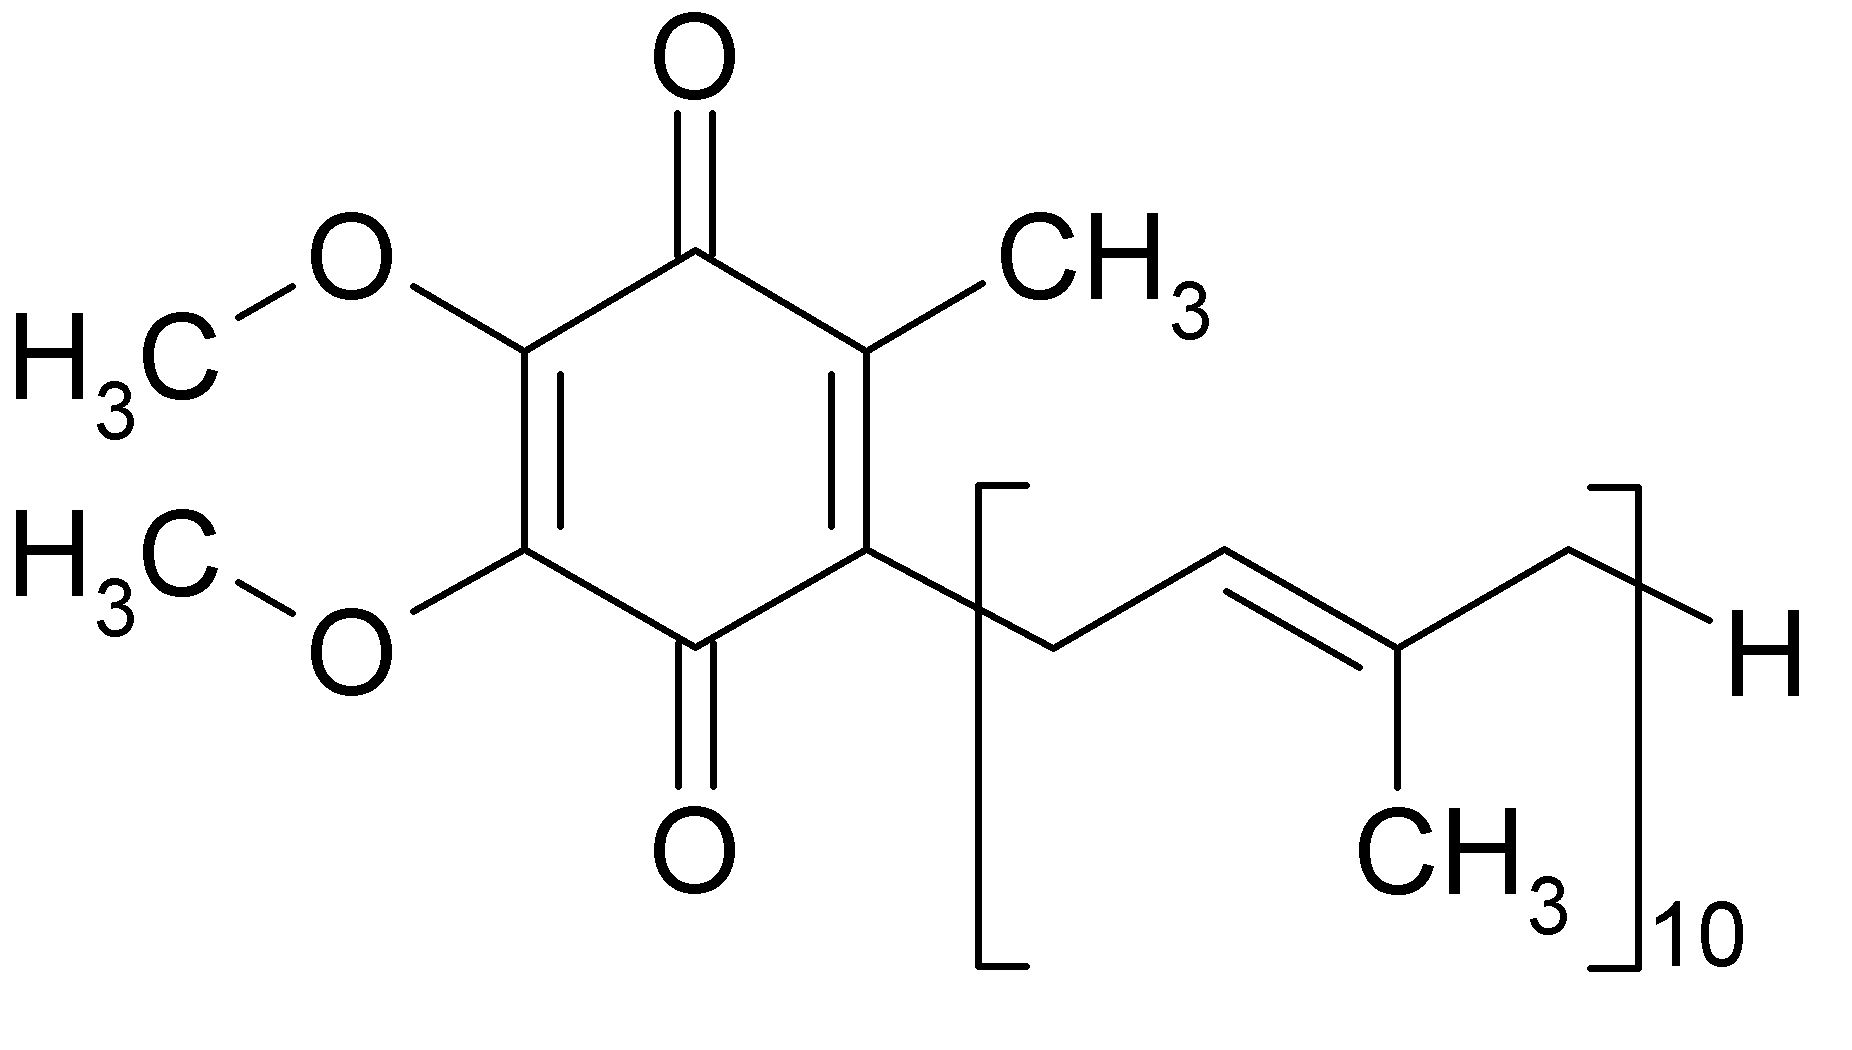
\includegraphics[width=14cm]{01-introduction/data/Ubiquinone.png}
	\caption[{Structure of the ubiquinone molecule.}]{{\bf Structure of the ubiquinone molecule.}
	\label{fig:Ubiquinone}}
	\end{center}
\end{figure}

In its oxidised form it is known as ubiquinone, whereas when reduced it is called ubiquinol. In the \Nm{} respiratory chain, ubiquinone is reduced to ubiquinol by the acceptance of 2 electrons from NADH (amongst others). Ubiquinol then donates electrons either directly to the terminal reductase NorB, or to the $bc_1$ complex.

\section{Respiration Regulatory Proteins in \Nm{}}
\subsection{NsrR - Nitrite Sensing Repressor Protein}
``NsrR is an NO-sensing Rrf2-type transcriptional repressor''\cite{Barth2009}. In \Nm{} (and \textit{N. gonorrhoeae}) it negatively regulates \textit{aniA} and \textit{norB}, and derepression is caused by NO\cite{Rock2007,Heurlier2008,Isabella2008}. Rrf2 proteins have two DNA-binding helix-helix domains\cite{Rock2007}, with a putative iron-sulfur cluster inbetween. The binding of the iron-sulfur cluster, which is expected to be by NO in NsrR, would perturb the structure of the repressor protein and prevent DNA binding\cite{Rock2007}.

\textit{norB} is expressed in a somewhat constitutive manner, in that with no repression \textit{norB} is still expressed to some extent\cite{Clark2010}. NsrR represses this expression until NO is present, at which point \textit{norB} can be expressed and the NorB enzyme can start removing the NO that is present.

\textit{aniA} is positively regulated by FNR, but this seems to be quite insensitive to oxygen in \Nm{}, thus \textit{aniA} would be expressed even at 60 to 80\% air saturation with oxygen\cite{Rock2007}. \textit{aniA} therefore needs to be corepressed in order to prevent it being expressed excessively in aerobic conditions.

\subsection{FNR - Fumarate and Nitrate Reductase Regulator}
Fumarate Nitrate Reductase is a transcriptional activator which binds to a 4Fe-4S cluster under anaerobic conditions. When oxygen concentrations are low, FNR causes increased expression of proteins that are necessary for anaerobic respiration. ``The presence of the 4Fe-4S cluster is correlated with protein dimerization, which enables it to bind promoter DNA''\cite{Edwards2010}. Four cysteine residues are believed to be ligated to the iron-sulfur cluster and these are required for FNR function. The oxygen sensitivity of FNR is achieved by the iron-sulfur cluster breaking down into 2Fe-2S via 3Fe-4S which is unable to bind DNA. In \Nm{}, \textit{aniA} expression is directly linked to the presence of FNR\cite{Rock2005}. When no NsrR is present, \textit{aniA} expression continues even up to 80\% oxygen saturation suggesting that FNR is actually quite insensitive to oxygen, an unusual response compared to FNR from \textit{E. coli}. FNR also becomes less sensitive to oxygen when it is bound to its cognate DNA\cite{Edwards2010}.

\subsection{NarQ/NarP - Nitrite Response Sensor/Regulator}
NarP and NarQ are a two component signal transduction pathway that regulate expression of \textit{aniA} in \textit{Neisseria}. NarQ is the sensor protein located in the inner membrane, while the regulator protein, NarP is found in the cytoplasm. Being a two component system, the sensor protein phosphorylates the regulator allowing it to bind the target DNA (which may consist of multiple sequences) to activate expression of genes.

In \textit{N. gonorrhoeae}, NarP was shown to enhance the expression of \textit{aniA} in response to the presence of nitrite, as a mutant lacking \textit{narP} was significantly slower at growing under denitrifiying conditions\cite{Overton2006}.

In \Nm{} expression of \textit{aniA} is increased greatly in conditions of high nitrite concentration\cite{Rock2005}. This effect is much more pronounced than simply being in oxygen limiting conditions. FNR appears to be required for \textit{aniA} expression even when NarP/NarQ are present\cite{Rock2005}. This suggests that the organism is intentionally preventing expression of nitrite reducing components until there is both a high concentration of nitrite \textit{and} a very low concentration of oxygen. This is plausible as even under oxygen limiting conditions oxygen reduction is still favoured over nitrite reduction.

\section{Organisation of Respiratory Chains in Other Bacteria}
The respiratory chain of \Nm{} is shown in a simplified form in Figure \ref{fig:nm_resp}. The components are coloured consistently throughout this section to allow easy comparison between the respiratory chains being discussed. As discussed previously, the respiratory chain of \Nm{} contains an initial electron donor, in this case NADH dehydrogenase. In fact there are a number of other electron donors, but they are not discussed here as NADH provides most of the electrons to the respiratory chain. There is also a quinone pool, consisting of ubiquinone/ubiquinol, intermediate \textit{c}-type cytochromes and terminal reductases.

\begin{figure}[tbp]
\begin{center}
	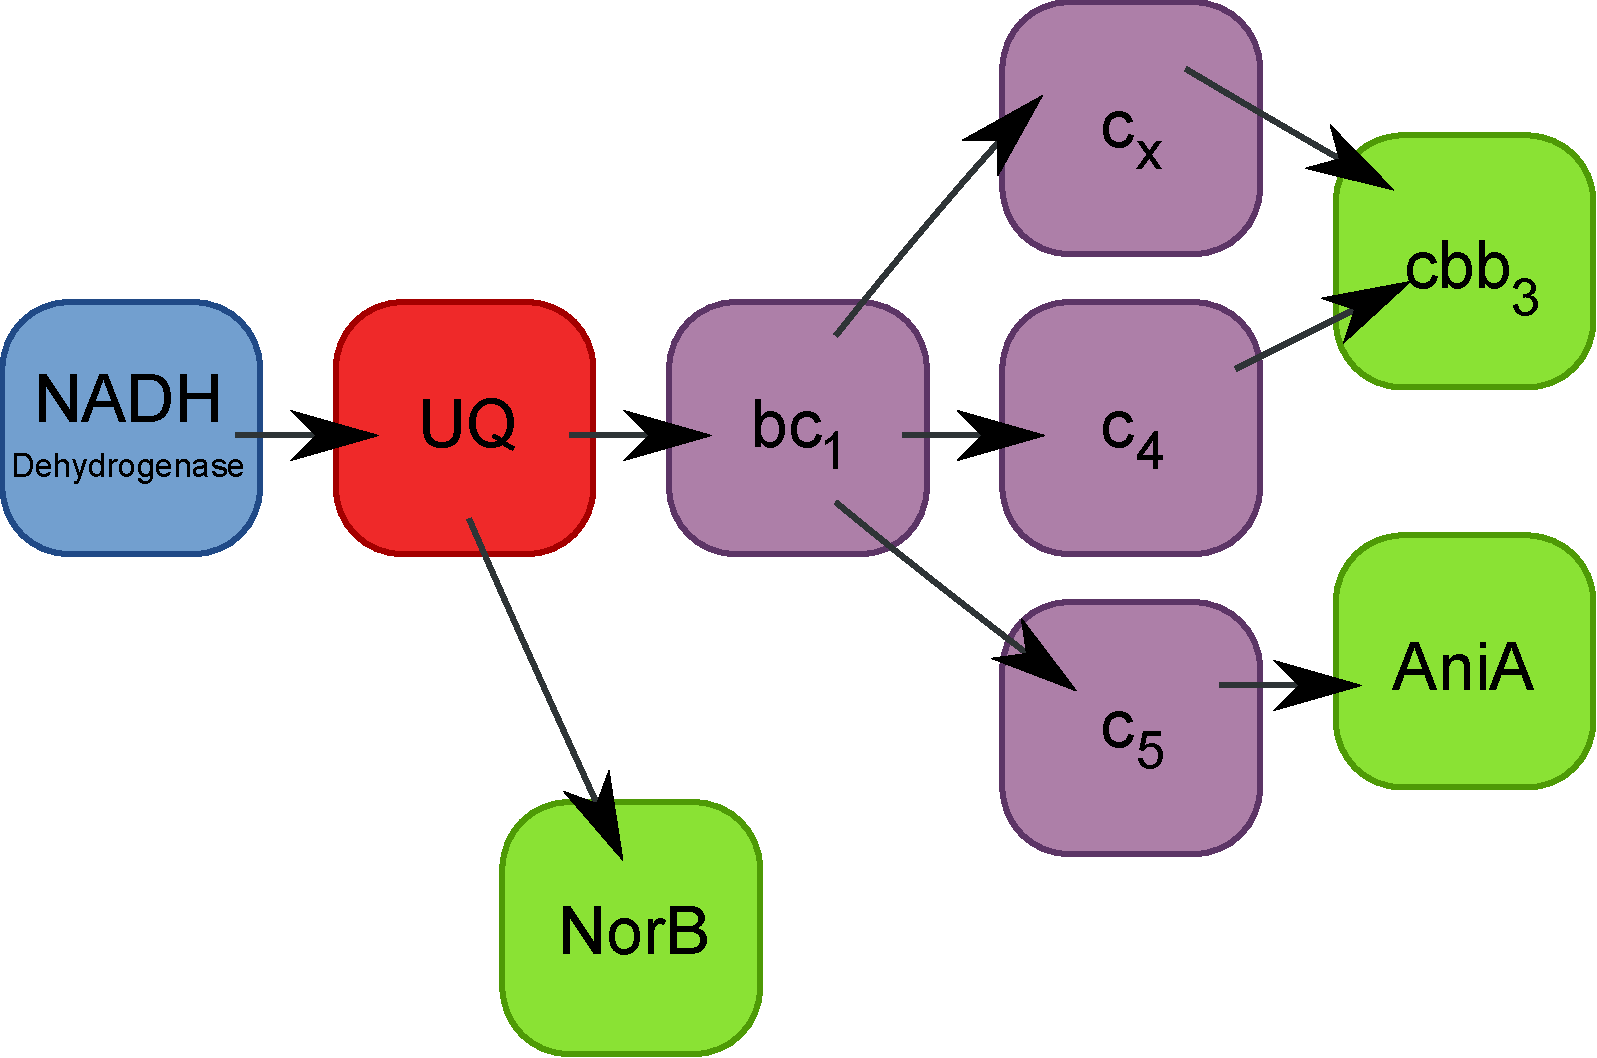
\includegraphics[height=9cm]{01-introduction/data/nm_resp.pdf}
	\caption[{Branched electron transport chains of \Nm{}.}]{{\bf Branched electron transport chains of \Nm{}.} Blue denotes initial electron donor, red denotes quinone pool, purple denotes cytochrome electron transporters and green denotes terminal reductases. UQ = ubiquinone.
	\label{fig:nm_resp}}
\end{center}
\end{figure}

\subsection{The Respiratory Chain of \textit{Paracoccus denitrificans}}
The respiratory chain of \textit{P. denitrificans} is shown in Figure \ref{fig:paracoccus_resp}. It is quite similar to that of \Nm{} with the exception of having a larger number of terminal reductases, and the ability to perform complete denitrification. The chain possesses an initial electron donor, a quinone pool, intermediate cytochrome electron transporters and terminal reductases.

The $bc_1$ complex of \Nm{} is present as an analogue (Ubiquinol-cyt \textit{c} oxidoreductase), and the chain includes 2 further downstream \textit{c}-type cytochromes. \textit{P. denitrificans} has 3 terminal oxygen reductases, $ba_3$, which oxidises the quinone pool directly, and \cbbthree{} and $aa_3$ which oxidise the \textit{c}-type cytochromes. All three oxygen reductases are HCOs. The branching of the aerobic electron transport chain is quite common among bacteria, but the reason for this is not currently fully understood.

The nitro-reductases found in \textit{P. denitrificans} are capable of complete denitrification as described in Figure \ref{fig:completedenitrification}. The nitrate reductases directly oxidise the quinone pool, whereas the nitrite and nitric oxide and nitrous oxide reductases oxidise the \textit{c}-type cytochromes instead.

As with \Nm{} there are a number of potential initial electron donors, but only NADH is shown for simplicity of comparison.

\begin{figure}[tbp]
\begin{center}
	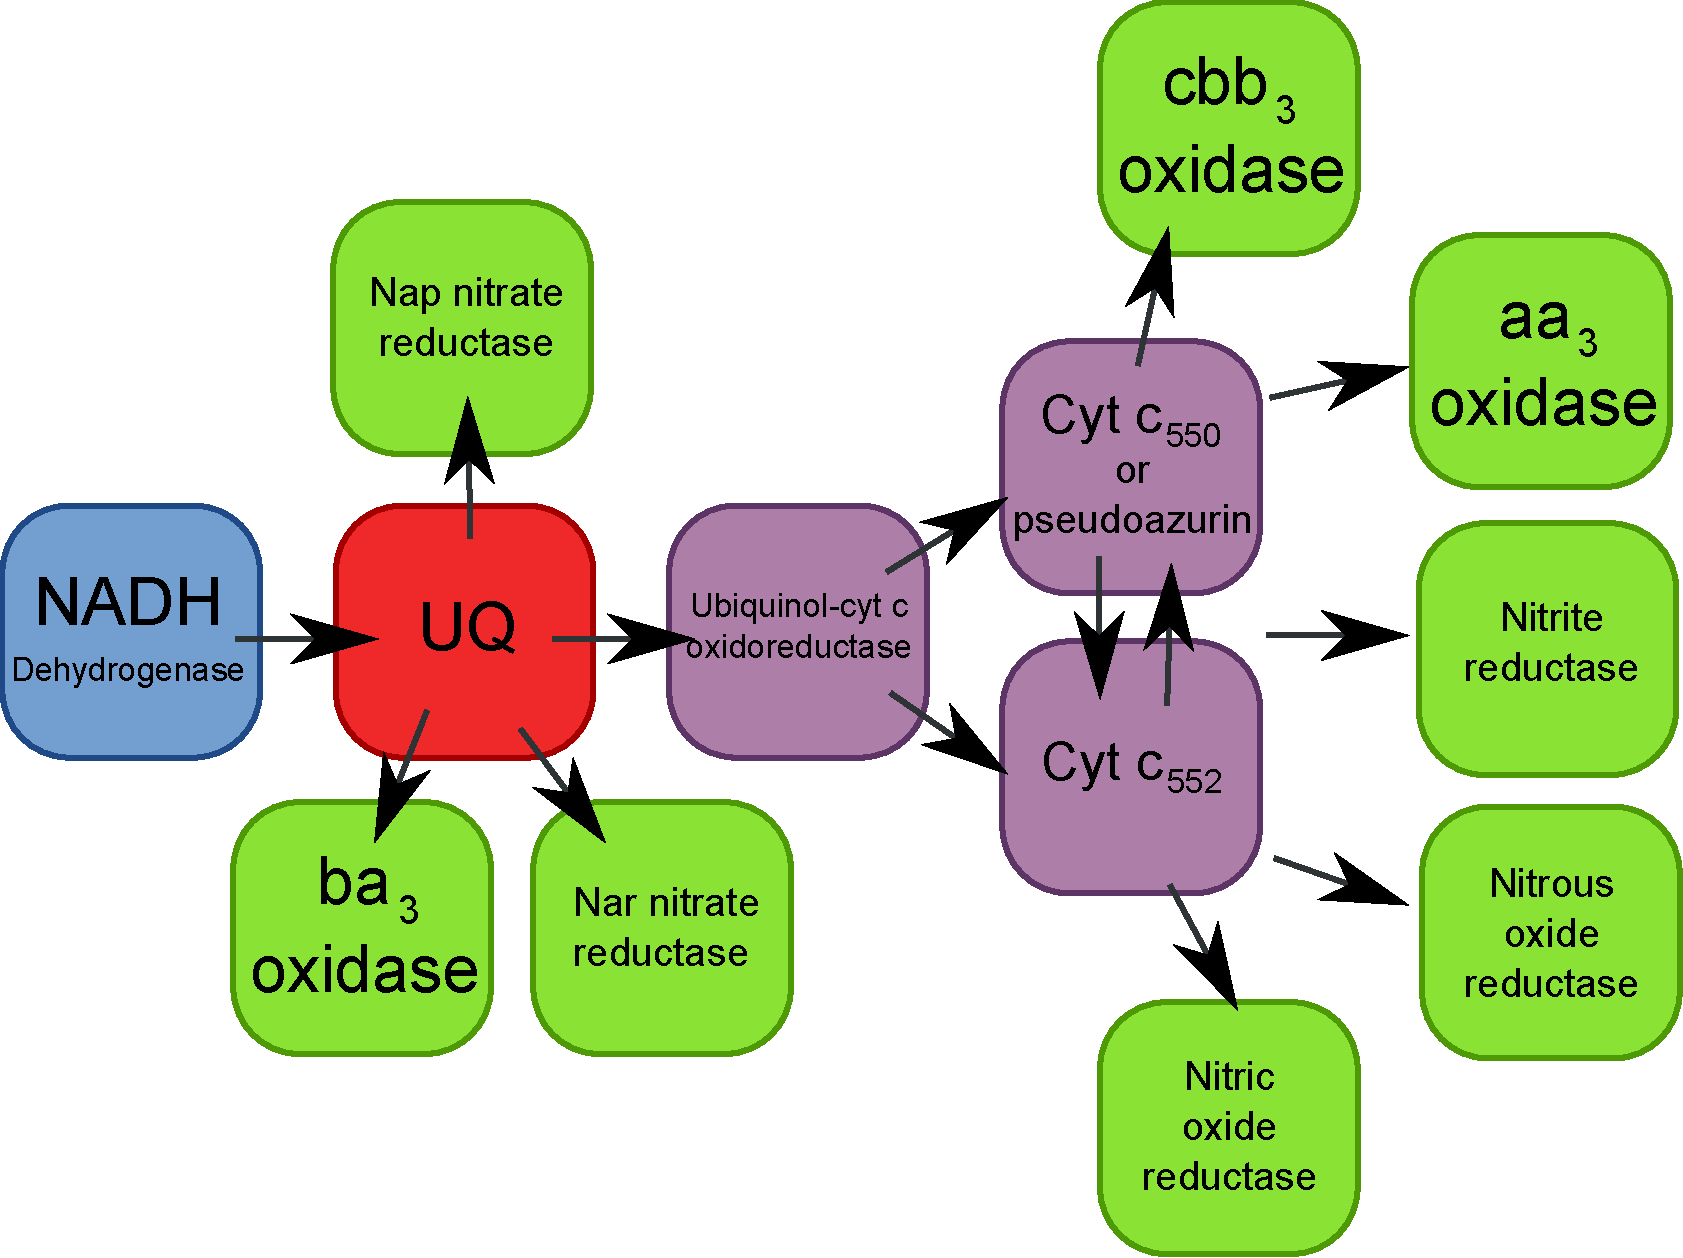
\includegraphics[height=9cm]{01-introduction/data/paracoccus_resp.pdf}
	\caption[{Branched electron transport chains of \textit{Paracoccus} species.}]{{\bf Branched electron transport chains of \textit{Paracoccus} species.} Blue denotes initial electron donor, red denotes quinone pool, purple denotes cytochrome electron transporters and green denotes terminal reductases. UQ = ubiquinone. Electron transfer between cytochromes $c_{552}$ and $c_{550}$ has not been demonstrated experimentally but is possible, given the redox potential of the proteins. Adapted from \citet{Baker1998}.
	\label{fig:paracoccus_resp}}
\end{center}
\end{figure}

\subsection{The Respiratory Chain of \textit{Escherichia coli}}
The respiratory chain of \textit{E. coli} is shown in Figure \ref{fig:e_coli_resp}. It can be seen to be quite distinct from other bacteria, and indeed from the mitochondrial respiratory chain. The most obvious difference between \textit{E. coli} and many other bacteria is the lack of \textit{c}-type cytochromes. The terminal reductases are able to be reduced directly by the quinone pool. Additionally, under anaerobic conditions, the quinone pool changes from being ubiquinone/ubiquinol to menaquinone/ubiquinol.

\textit{E. coli} also has a number of different terminal reductases in the form of cyt $bo_3$ and cyt \textit{bd}. Cyt $bo_3$ is an HCO and is structurally very similar to cyt $aa_3$. Cyt \textit{bd} shows no sequence similarity with the HCO superfamily and has no $\mathrm{Cu}_\mathrm{B}$ site. Cyt \textit{bd} has a much higher affinity for oxygen than cyt $bo_3$ so is synthesised at low oxygen concentration.

\textit{E. coli} is also capable of partial denitrification and possesses enzymes to reduce nitrate and nitrite, which are also under the regulatory control of FNR. The reduction of nitrite differs from \Nm{} and \textit{P. denitrificans} as $\mathrm{NO}_2^-$ is not reduced to NO, but to $\mathrm{NH}_4^+$ instead.

As with \Nm{} and \textit{P. denitrificans} there are a number of potential initial electron donors, but only NADH is shown for simplicity of comparison.

\begin{figure}[tbp]
\begin{center}
	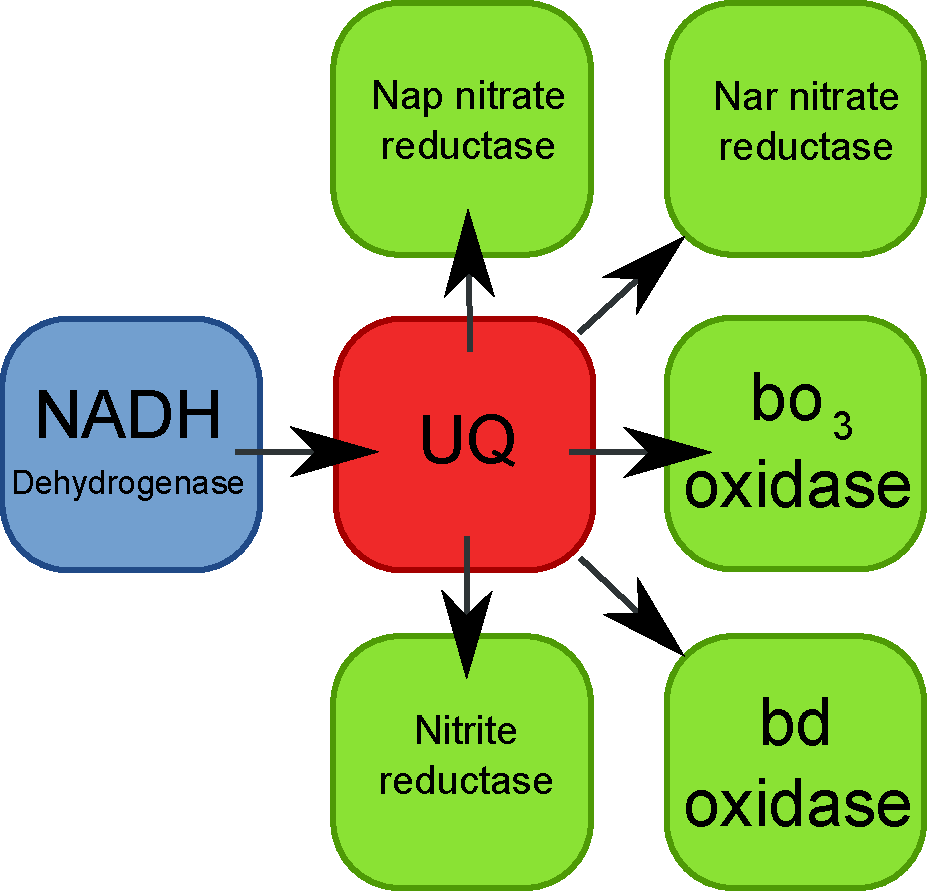
\includegraphics[height=9cm]{01-introduction/data/e_coli_resp.pdf}
	\caption[{Branched electron transport chains of \textit{E. coli}.}]{{\bf Branched electron transport chains of \textit{E. coli}.} Blue denotes initial electron donor, red denotes quinone pool and green denotes terminal reductases. UQ = ubiquinone. Under anaerobic conditions, ubiquinone is replaced by menaquinone. Adapted from \citet{Nicholls1992}.
	\label{fig:e_coli_resp}}
\end{center}
\end{figure}


\section{Systems Biology}
Systems biology is the process of ``studying biological systems in their whole [...], reinforced by high throughput [...] molecular tests and considerable sophistication in computational modelling''\cite{Kahlem2006}. Systems biology ``combines approaches and methods from systems engineering, computational biology, statistics, genomics, molecular biology, biophysics and other fields''\cite{Doyle2006}.

The aim of Systems biology is to take our detailed understanding of organisms beyond the molecular and cellular level. These are the levels to which the disciplines of molecular and biology and biochemistry (among others) are more suited. It aims to take our understanding to the level of the entire ``complex system''. Which is to say we gain understanding into the way the organism behaves as a whole, rather than just having knowledge of the individual parts.

The level of complexity in biological systems is far greater than the popular notion of what defines a complex system, however. Biological systems consist of multiple different individual elements each performing specific tasks interacting with each other to create 'coherent' behaviour. This is very different from popular complex systems which are collections of simple, identical components interacting to produce 'complex' behaviour\cite{Kitano2002}.

Gaining understanding such a complex system is difficult, and Kitano suggests that it requires insight into the following properties\cite{Kitano2002a}:
\begin{enumerate}
 \item {\bf Structure of the system.} This includes the way the system interactions are ``laid out'' both at a component level and an organismal level.
 \item {\bf The dynamics of the system.} This involves understanding how the organism behaves under any given conditions over a particular time period. This may include understanding how the metabolic processes change under these conditions etc.
 \item {\bf How the system is controlled.} The control mechanisms can be tailored to suit the desired function or to minimised the chance of malfunction.
 \item {\bf How the system is designed.} ``Trial and error'' experimentation can be done away with, as the system can be designed based on defined properties, backed up by models and simulations.  
\end{enumerate}

The level of integration between systems biology approaches and experimentation can be seen in Figure \ref{fig:systems-biology}. This shows the iterative cycles that are necessary to gain understanding in both areas. The experimentation provides data to refine and develop the system model, and data from that model can go on to improve the design of the experiment.

\begin{figure}[tbp]
 \begin{center}
 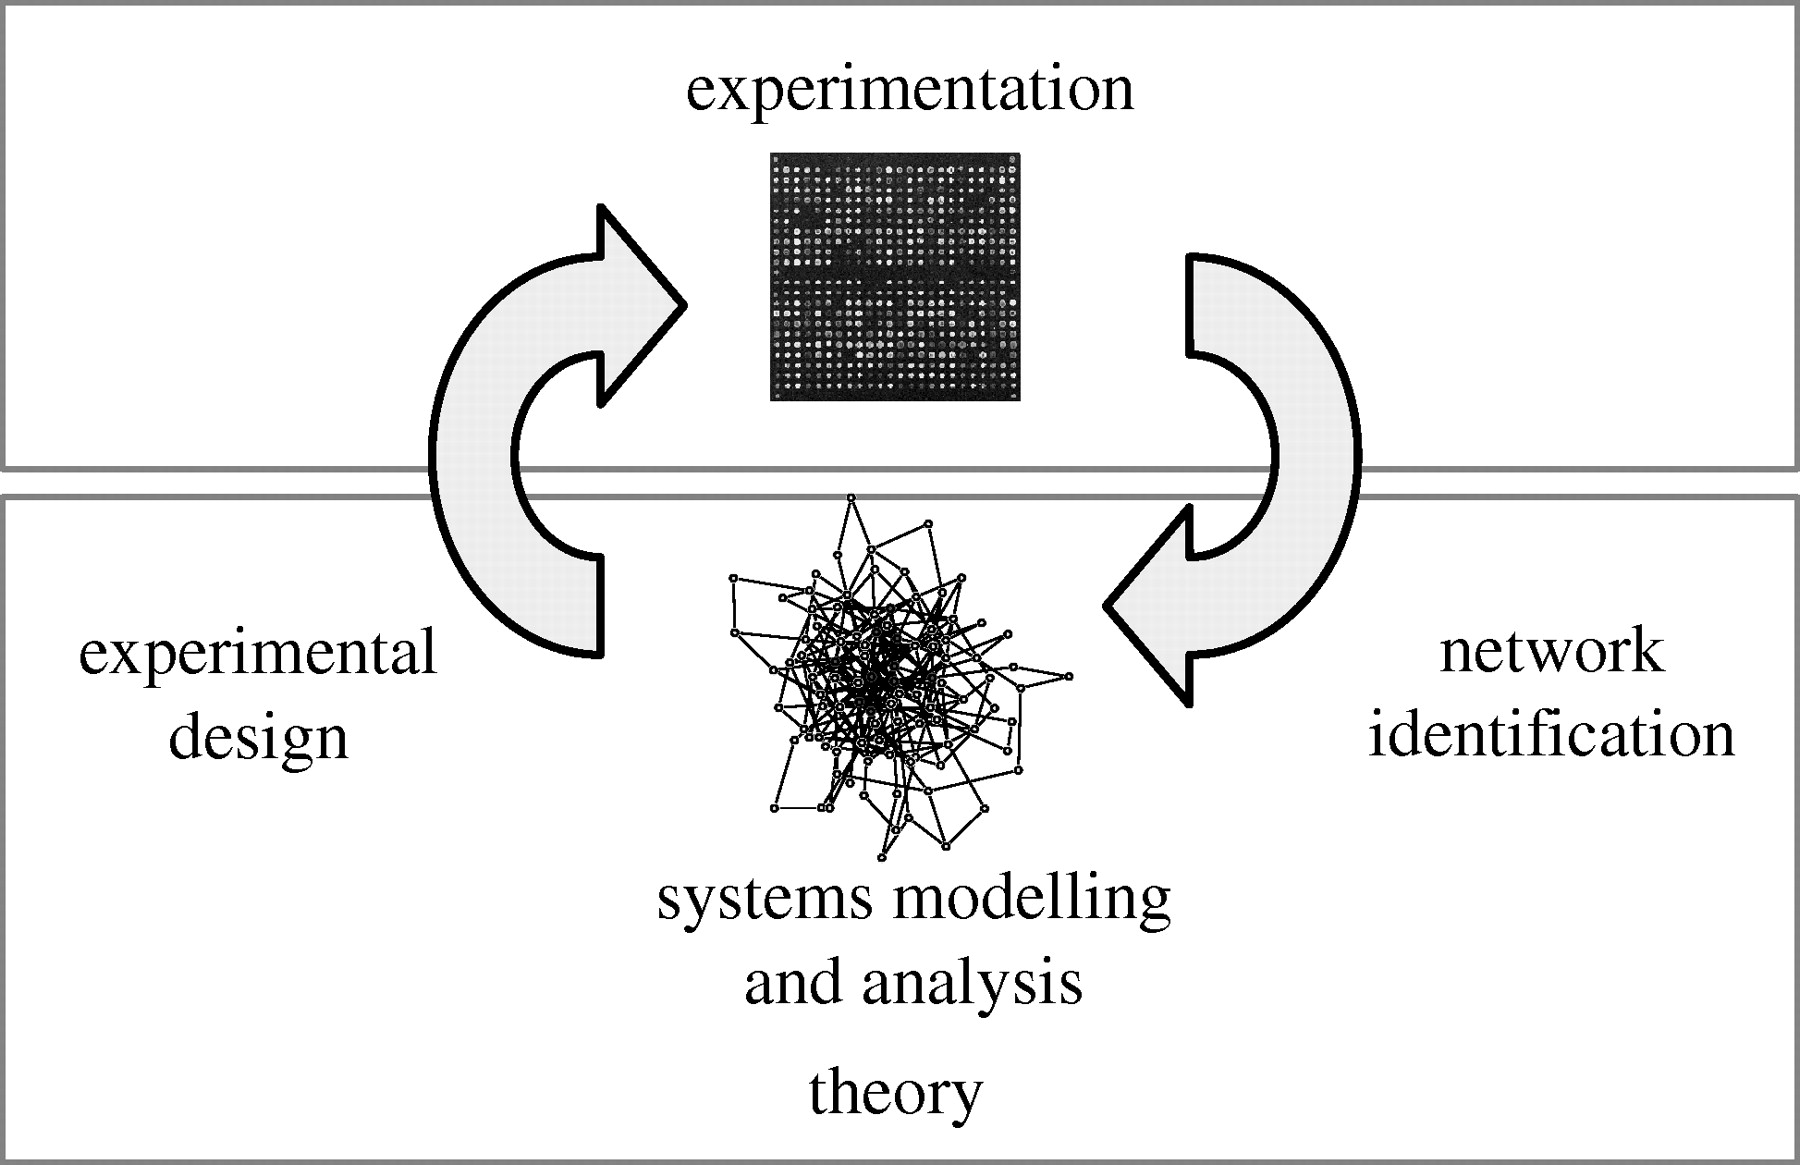
\includegraphics[width=14cm]{./01-introduction/data/F1.png}
 % F1.png: 1800x1165 pixel, 300dpi, 15.24x9.86 cm, bb=0 0 432 280
\end{center}
%This caption requires notocite otherwise the citation always gets number 1
\caption[{Systems biology cycle.}]{{\bf Systems biology cycle.} Interactions between experimental analysis and theoretical approaches, and the main tasks for theory at the interfaces. \protect\citet{Doyle2006}
\label{fig:systems-biology}}
\end{figure}

Systems biology extends further into a computational discipline when you consider that if you can create a model of a system, you can potentially run a simulation of the system using the model. Simulations can be developed for multiple stages of the process, from molecular to organismal. Simulations of interactions based on gene regulatory network models are being studied\cite{Valencia2002}, as are complete plant development models\cite{Mundermann2005,Prusinkiewicz2004,Prusinkiewicz2006}.

\begin{figure}[tbp]
 \centering
 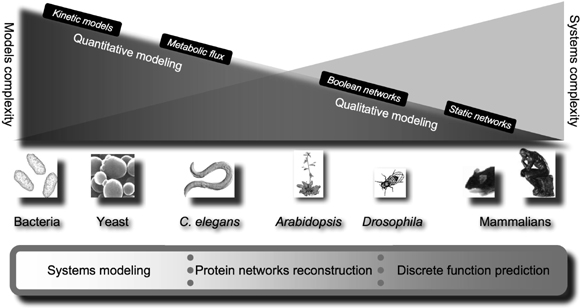
\includegraphics[width=14cm]{./01-introduction/data/msb4100080-f1.png}
 % msb4100080-f1.png: 580x308 pixel, 125dpi, 11.79x6.26 cm, bb=0 0 334 177
\caption[{System complexity.}]{{\bf System complexity.} Diagram showing how system complexity varies across organisms, and how the complexity of the models we can produce is currently the inverse of systems complexity. \citet{Kahlem2006}
\label{fig:systems-power}}
\end{figure}

Figure \ref{fig:systems-power} shows one of the limitations of the current technology ``powering'' systems biology. As organisms get more complex, the models we can produce get less complex and less quantitative\cite{Kahlem2006}. This concomitant lack of data in models of complex organisms decreases the likelihood of being able to produce a simulation of the model. We might be able to simulate \textit{aspects} of a complex organism, such as the human heart\cite{Crampin2004} but we are still a long way from being able to simulate the entire human body.

For simpler systems, like yeast, or \textit{E. coli} an enormous amount of data already exists about individual gene regulation, protein interactions etc. and it is possible to build sophisticated models of the entire gene regulatory network and more\cite{Barabasi2004,Peercy2006}.

A systems biology approach to understanding the mechanism of respiration in \Nsm{} is necessary as there are a number of components in the system which are inherently unmeasurable.

\section{Modelling}

\subsection{Modelling Respiratory Systems}

A limited amount of modelling has been carried out on bacterial respiratory chains, these focused on the denitrification pathway and treated the pathway as a simple electrical circuit\cite{Almeida1997}. An alternative approach involved modelling respiration using ``P systems'' which are probabilistic models of events. This assigned a probability of each reaction happening, dependant on the state of the system and then iterated through a given set of steps evaluating probabilities and altering values based on the outcome\cite{Cavaliere2006}. This approach to modelling was limited in that it was only predicting the quantities of 1 component in each of 2 ``compartments''; oxygen in the cell membrane and carbon dioxide in the thylakoid membrane (the model was developed using cyanobacteria).

Some modelling of parts of the respiratory chain in \textit{E. coli} have also been modelled. \citet{Peercy2006} created a kinetic model of how cytochrome production is regulated by oxygen using differential equations. They created a set of differential equations to describe the relevant reactions and then populated the model using parameters gathered from the literature.

Since when modelling respiration in a cell, the most important factor is the change in concentration of components over time without any particular spatial constraints, ordinary differential equations (ODEs)\nomenclature{ODE}{Ordinary Differential Equation} are an appropriate technique. In these systems the model does not change with regard to the spatial arrangement of any of the components. If the system requires changes in time \textit{and} space, then partial differential equations (PDEs)\nomenclature{PDE}{Partial Differential Equation} would be necessary (and more complicated)\cite{Klipp2005}.

Ordinary differential equations only depend on one variable; the time ($t$). In this case, the change in concentration over time for each component can be modelled as a single differential equation. For multiple components this leads to multiple differential equations with some that rely on the result of another (if the rate of one reaction is directly related to the concentration of another component). These ODEs must then be solved in parallel at a suitable time-scale.

Complications arise when using differential equations if the processes are considered to be stochastic, as a differential equation model assumes that every component can have a continuous value, which is not the case as molecules are discrete. However if the system being modelled is sufficiently large, this effect can be ignored. If the reaction component size is small ($<$ 100s of molecules) stochastic simulation algorithms have to be used as described by \citet{Gillespie1977}. This method requires far more computation than solving ODEs, as the model will spend most of its time calculating values for reactions involving large molecules even though this is not necessary as the reaction is not stochastic. Additionally, the time interval used between reaction steps is usually very small, meaning the simulation progresses slowly\cite{Klipp2005}.

\subsection{Modelling Tools}

A number of software packages exist that are capable of this type of modelling such as the Systems Biology Workbench\cite{Sauro2003} and COPASI\cite{Hoops2006}. These allow you to enter biochemical reactions in a format familiar to biologists, and have pre-defined libraries for types of reactions such as mass-action, or one with Michaelas-Menton kinetics etc. The mathematical equations are then derived automatically from the reactions and can be modified by hand if necessary. Parameters for the mathematical equations must be entered, and these will usually be derived from experimental data, or in some cases educated guesses (at least initially). Once a parameter set has been created, the modelling software can run a time-course using a relevant solver-algorithm. COPASI includes 4 solvers,  LSODA (Livermore Solver for Ordinary Differential Equations)\cite{Radhakrishnan1993} for deterministic systems (such as ODEs), Gibson-Bruck\cite{Gibson2000} for stochastic systems and Runge-Kutta and LSODA for hybrid systems (where portions are not considered to be stochastic).

\section{Aims}
The over-arching aim of this study was to produce a working mathematical model of the respiratory system of \Nm{} which has been refined and parametrised by experimental biological data. This mathematical model should be able to accurately simulate experimental datasets with known outcomes, and also be able to predict the outcome of experiments that have not been performed. This model, will also be able to provide insight into the states of various components throughout the respiratory process, such as enzymatic oxidation states, some of which are very difficult, if not impossible, to obtain in an \textit{in vivo} study.

The layout of \Nm{} respiratory chain, even though it is longer than that of the model organism \textit{Escherichia coli} is more similar to most other bacteria. This, along with its profound medical importance make it an excellent target for the type of mathematical modelling described above.

The individual aims of the study are therefore:
\begin{enumerate}
\item {\bf Construct a mathematical model of the \Nm{} respiratory chain.} This will involve the conversion of the kinetic reactions involved in respiration into mathematical equations that can be linked together, and if justified simplifying the chain.
\item {\bf Obtaining experimental data on respiratory rates and enzyme kinetics.} This will involve performing experiments on respiring \Nm{} and recording the concentrations of respiratory substrates under different conditions.
\item {\bf Parametrise the model using experimental data.} To do this a system will need to be developed which can iteratively fit experimental data to specific parts of the mathematical model.
\end{enumerate}